% Homework template for Inference and Information
% UPDATE: September 26, 2017 by Xiangxiang
\documentclass[a4paper]{article}
\usepackage{ctex}
\usepackage{amsmath, amssymb, amsthm}
\usepackage{moreenum}
\usepackage{mathtools}
\usepackage{url}
\usepackage{bm}
\usepackage{enumitem}
\usepackage{graphicx}
\usepackage{listings}
\usepackage{color}

\lstset{
    basicstyle          =   \sffamily,          % 基本代码风格
    keywordstyle        =   \bfseries,          % 关键字风格
    commentstyle        =   \rmfamily\itshape,  % 注释的风格,斜体
    stringstyle         =   \ttfamily,  % 字符串风格
    flexiblecolumns,                % 别问为什么,加上这个
    numbers             =   left,   % 行号的位置在左边
    showspaces          =   false,  % 是否显示空格,显示了有点乱,所以不现实了
    numberstyle         =   \zihao{-5}\ttfamily,    % 行号的样式,小五号,tt等宽字体
    showstringspaces    =   false,
    captionpos          =   t,      % 这段代码的名字所呈现的位置,t指的是top上面
    frame               =   lrtb,   % 显示边框
}

\lstdefinestyle{Python}{
    language        =   Python, % 语言选Python
    basicstyle      =   \zihao{-5}\ttfamily,
    numberstyle     =   \zihao{-5}\ttfamily,
    keywordstyle    =   \color{blue},
    keywordstyle    =   [2] \color{teal},
    stringstyle     =   \color{magenta},
    commentstyle    =   \color{red}\ttfamily,
    breaklines      =   true,   % 自动换行,建议不要写太长的行
    columns         =   fixed,  % 如果不加这一句,字间距就不固定,很丑,必须加
    basewidth       =   0.5em,
}
\usepackage{subcaption}
\usepackage{booktabs} % toprule
\usepackage[mathcal]{eucal}
\usepackage[thehwcnt = 2]{iidef}

\thecourseinstitute{清华大学电子工程系}
\thecoursename{\textbf{媒体与认知} \space 课堂2}
\theterm{2021-2022学年春季学期}
\hwname{作业}
\begin{document}
\courseheader
\name{郭中贺}
\vspace{3mm}
\centerline{\textbf{\Large{理论部分}}}

\section{单选题(15分)}
\subsection{\underline{D}}

\subsection{\underline{C}}

\subsection{\underline{B}}

\subsection{\underline{C}}

\subsection{\underline{D}}

\section{计算题(15 分)}
\subsection{设隐含层为$\mathbf{z}=\mathbf{x}\mathbf{W}^T+\mathbf{b}$,其中$\mathbf{x}\in R^{(1 \times m)}$,$\mathbf{z}\in R^{(1\times n)}$,$\mathbf{W}\in R^{(n\times m)}$,$\mathbf{b} \in R^{(1\times n)}$均为已知,其激活函数如下:
$$\mathbf{y}=\tanh(\mathbf{z})=\frac{e^\mathbf{z}-e^{-\mathbf{z}}}{e^\mathbf{z}+e^{-\mathbf{z}}}$$
若训练过程中的目标函数为L,且已知L对$\mathbf{y}$的导数 $\frac{\partial L}{\partial \mathbf{y}}=[\frac{\partial L}{\partial y_1},\frac{\partial L}{\partial y_2},...,\frac{\partial L}{\partial y_n}]$和$\mathbf{y}=[y_1,y_2,...,y_n]$的值。
}
\subsubsection{请使用$\mathbf{y}$表示出$\frac{\partial \mathbf{y}}{\partial \mathbf{z}}$
}
经过计算可得到
$$
\frac{\partial y_i}{\partial z_j} = 
    \left\{ 
        \begin{array}{lcl}
        0, & &i \neq j\\
        \frac{4}{\left( e^{z_j}+e^{-z_j} \right)^2}, & &i = j
        \end{array}
    \right.
$$

%$$
%\frac{\partial \mathbf{y}}{\partial \mathbf{z}} = 
%\frac{4}{\left( e^\mathbf{z}+e^{-\mathbf{z}} \right)^2}
%$$
另一方面
$$
y_i^2 = 1-\frac{4}{\left( e^{z_i}+e^{-z_i} \right)^2}
$$

因此,可求得$\frac{\partial y_i}{\partial z_i} = 1-y_i^2$

\subsubsection{请使用$\mathbf{y}$和$\frac{\partial L}{\partial \mathbf{y}}$表示$\frac{\partial L}{\partial \mathbf{x}}$,$\frac{\partial L}{\partial \mathbf{W}}$,$\frac{\partial L}{\partial \mathbf{b}}$。
}
提示:$\frac{\partial L}{\partial \mathbf{x}}$,$\frac{\partial L}{\partial \mathbf{W}}$,$\frac{\partial L}{\partial \mathbf{b}}$与x,W,b具有相同维度。\par
$$
\frac{\partial L}{\partial \mathbf{x}} = 
\sum_{i=1}^n \frac{\partial L}{\partial z_i} * 
\frac{\partial z_i}{\partial \mathbf{x}} = 
\frac{\partial L}{\partial \mathbf{z}}\cdot \mathbf{W}
$$

其中
$$
\frac{\partial L}{\partial z_i} = \frac{\partial L}{\partial y_i}*
\frac{\partial y_i}{\partial z_i} = \frac{\partial L}{\partial y_i} * (1-y_i^2)
$$
因此
$$
\frac{\partial L}{\partial \mathbf{z}} = 
\frac{\partial L}{\partial \mathbf{y}}* (1-\mathbf{y}^2)
$$
$$
\frac{\partial L}{\partial \mathbf{x}} = \left(
\frac{\partial L}{\partial \mathbf{y}}* (1-\mathbf{y}^2)
\right)\cdot \mathbf{W}
$$
上式中的*和平方均代表向量中的对应元素运算,$\cdot$表示矩阵(向量)乘法.
同理可得:
$$
\frac{\partial L}{\partial \mathbf{W}} = 
\sum_{i=1}^n \frac{\partial L}{\partial z_i} * 
\frac{\partial z_i}{\partial \mathbf{W}} = \left(
\frac{\partial L}{\partial \mathbf{z}}  \right)^T \cdot \mathbf{x}=
\left( \frac{\partial L}{\partial \mathbf{y}}* (1-\mathbf{y}^2) \right)^T
\cdot \mathbf{x}
$$

$$
\frac{\partial L}{\partial \mathbf{b}} = 
\sum_{i=1}^n \frac{\partial L}{\partial z_i} * 
\frac{\partial z_i}{\partial \mathbf{b}} = 
\frac{\partial L}{\partial \mathbf{z}} =\frac{\partial L}{\partial \mathbf{y}}* (1-\mathbf{y}^2)
$$

\vspace{6mm}
\centerline{\textbf{\Large{编程部分}}}
\vspace{3mm}
% 请根据是否选择自选课题的情况选择“编程作业报告”或“自选课题开题报告”中的一项完成
\section{编程作业报告}

\subsection{训练模型}
\subsubsection{SGD优化器默认参数}
运行 python recognition.py --mode train 训练模型后,
控制台输出结果与loss变化曲线分别如图1、2所示。\par
\begin{figure}[hp]
    \centering
    \begin{minipage}{0.48\textwidth}
        \centering
        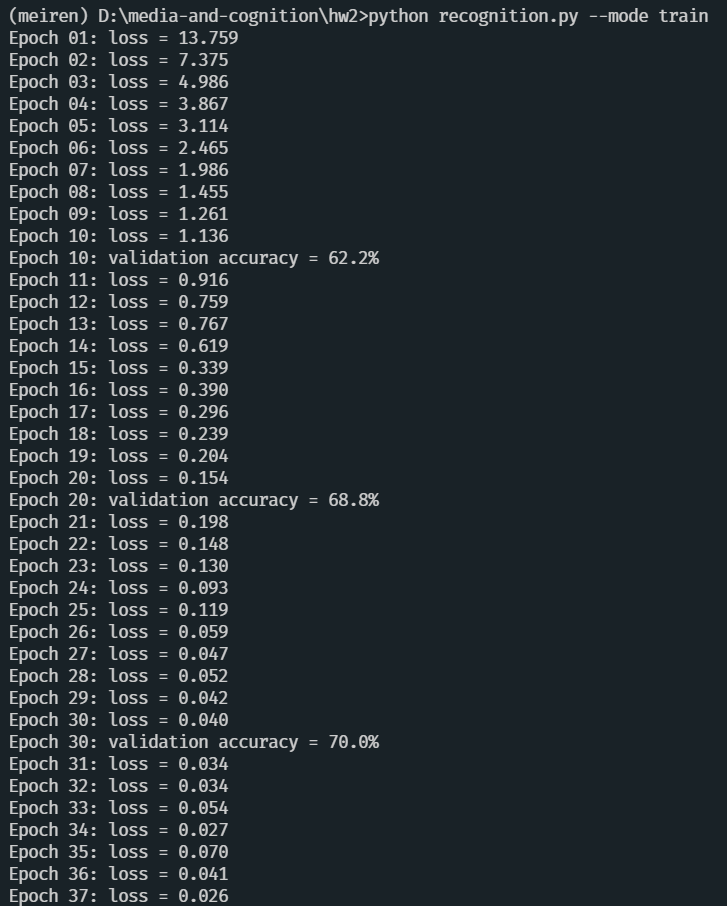
\includegraphics[width=5cm]{image/train_cmd.png}
    \end{minipage}
    \begin{minipage}{0.48\textwidth}
        \centering
        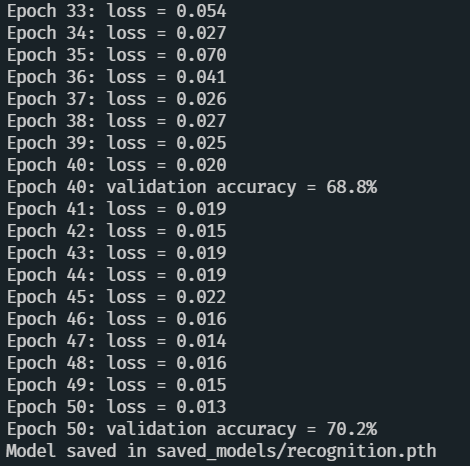
\includegraphics[width=5cm]{image/train_cmd2.png}
    \end{minipage}
    \caption{cmd输出结果}
    \vspace{-1cm}
\end{figure}

\begin{figure}[hp]
    \centering
    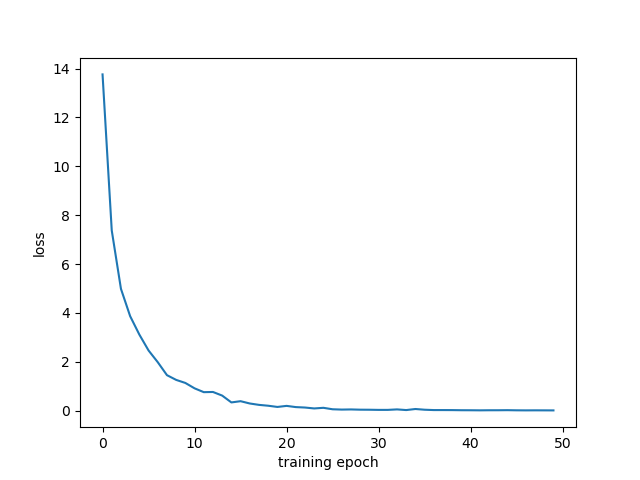
\includegraphics[width=8cm]{image/train_figure.png}
    \caption{loss曲线}
\end{figure}
结果分析:由图3曲线可知,一开始训练的loss较高,约为14。
随着训练轮数的增加,loss逐渐下降,最终稳定到0.015左右。
另一方面,由图2输出,可知模型在验证集上的准确率为70\%左右,并且随着训练轮数增加
准确率有小幅度上升。但是由于数据集数量过少,因此最终训练后准确率并不太高。
\subsubsection{Adam优化器并修改参数}
运行 
python recognition.py --mode train --hsize 64 --lr 2e-3 --optim\_type adam --momentum 0 --weight\_decay 0.1
训练模型后,
控制台输出结果与loss变化曲线分别如图3、4所示。\par
\begin{figure}[hp]
    \centering
    \begin{minipage}[t]{0.48\textwidth}
        \centering
        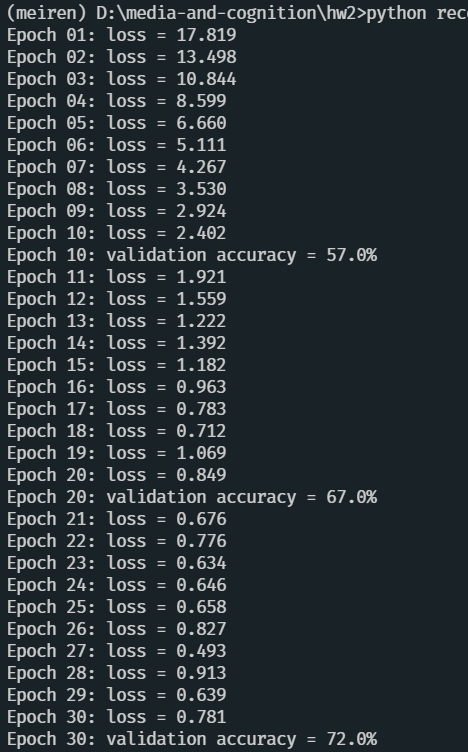
\includegraphics[width=5cm]{image/adam_cmd1.png}
        \end{minipage}
        \begin{minipage}[t]{0.48\textwidth}
        \centering
        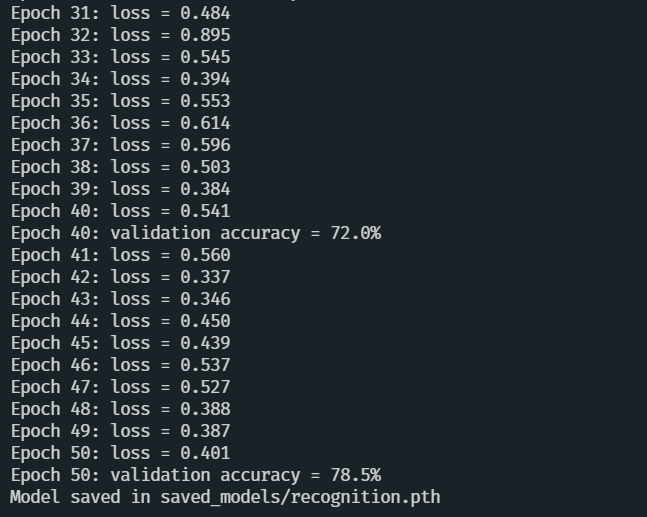
\includegraphics[width=5cm]{image/adam_cmd2.png}
    \end{minipage}
    \caption{cmd输出结果}
    \vspace{-1cm}
\end{figure}

\begin{figure}[htbp]
    \centering
    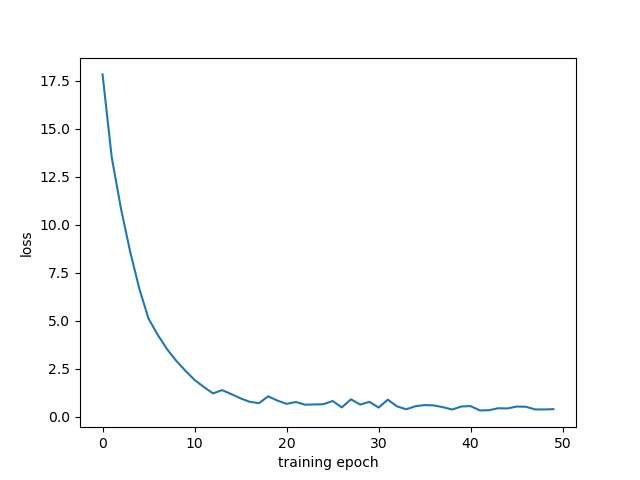
\includegraphics[width=8cm]{image/adam_figure.png}
    \caption{loss曲线}
\end{figure}
通过对比可以看出,使用adam优化器后,训练的整体loss略有上升,但是训练的最终
准确率有一定幅度的提高,提高到了78\%左右,因此,最终决定使用adam优化器和相应参数。

\subsection{测试模型及可视化}
运行 python recognition.py --mode test 验证模型,
控制台输出结果如图5所示。\par
\begin{figure}[hp]
    \centering
    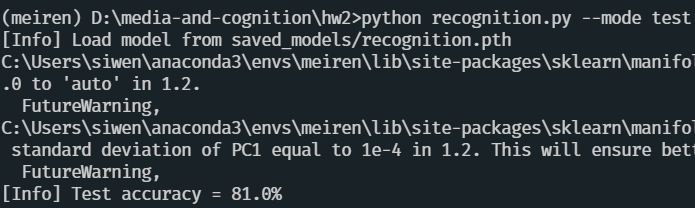
\includegraphics[width=8cm]{image/test_cmd.png}
    \caption{cmd输出结果}
\end{figure}
可见使用训练50轮之后的模型,在测试集上进行测试,其准确率更高达到了81.0\%。
可见,该训练模型并不只能识别用于训练和验证的数据,具有一定的泛用性。\par
可视化分类结果如图6所示。\par
\begin{figure}[hp]
    \centering
    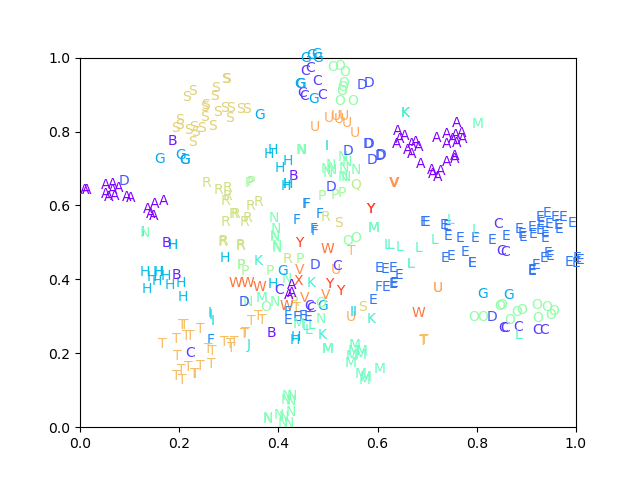
\includegraphics[width=10cm]{image/test_figure.png}
    \caption{可视化结果}
\end{figure}
通过分析比较,我们可以看出:部分字母可以较好地分辨出来,比如左上角的S、R,右侧的E、O,左下角的T等。
但是也有很多字母分辨性能较差,如C和G容易混淆。
其主要原因,还是训练的数据集样本过少,不能很好地训练出各个字母的特征,模型也就无法分辨出不同字母。
\subsection{预测图像类别}
此步骤使用adam优化器训练后的模型recognition.pth,
输入样本为提供的predict01.png(字母A)和predict02.png(字母B)。
预测结果分别如下。图7为predict01.png预测结果,图8为predict02.png预测结果。\par
\begin{figure}[hp]
    \centering
    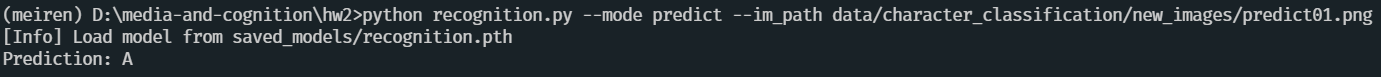
\includegraphics[width=10cm]{image/pred01.png}
    \caption{predict01.png预测结果}
\end{figure}
\begin{figure}[hp]
    \centering
    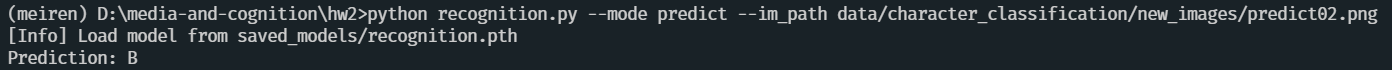
\includegraphics[width=10cm]{image/pred02.png}
    \caption{predict02.png预测结果}
\end{figure}
可见这两张图片的预测结果十分准确。
\subsection{本次作业遇到的问题及解决方法}
无。
\subsection{对本次作业的意见及建议}
本次作业也较为简单,通过代码注释中的一步一步教程,
我们能很快了解下一步该做什么,该如何实现。我的建议
是也可以试着让同学们自己编写一个自定义激活函数以达到练习的目的。
\end{document}



%%% Local Variables:
%%% mode: late\rvx
%%% TeX-master: t
%%% End:
